\documentclass[tikz,border=10pt]{standalone}
\usepackage{tikz}
\usetikzlibrary{shapes.geometric, arrows.meta, positioning, calc, fit, backgrounds}
\usepackage{amsmath,amssymb}
\usepackage{xcolor}

% Unified Academic Color Palette
\definecolor{cInput}{RGB}{235, 248, 255}
\definecolor{bInput}{RGB}{49, 130, 206}

\definecolor{cTrans}{RGB}{240, 249, 255}
\definecolor{bTrans}{RGB}{43, 108, 176}

\definecolor{cGCN}{RGB}{230, 255, 250}
\definecolor{bGCN}{RGB}{49, 151, 149}

\definecolor{cRecurr}{RGB}{250, 245, 255}
\definecolor{bRecurr}{RGB}{128, 90, 213}

\definecolor{cHead}{RGB}{255, 245, 245}
\definecolor{bHead}{RGB}{229, 62, 62}

\definecolor{cFusion}{RGB}{254, 252, 191}
\definecolor{bFusion}{RGB}{214, 158, 46}

\definecolor{cGray}{RGB}{247, 250, 252}
\definecolor{bGray}{RGB}{160, 174, 192}

\definecolor{tDark}{RGB}{26, 32, 44}
\definecolor{tMuted}{RGB}{74, 85, 104}

\begin{document}
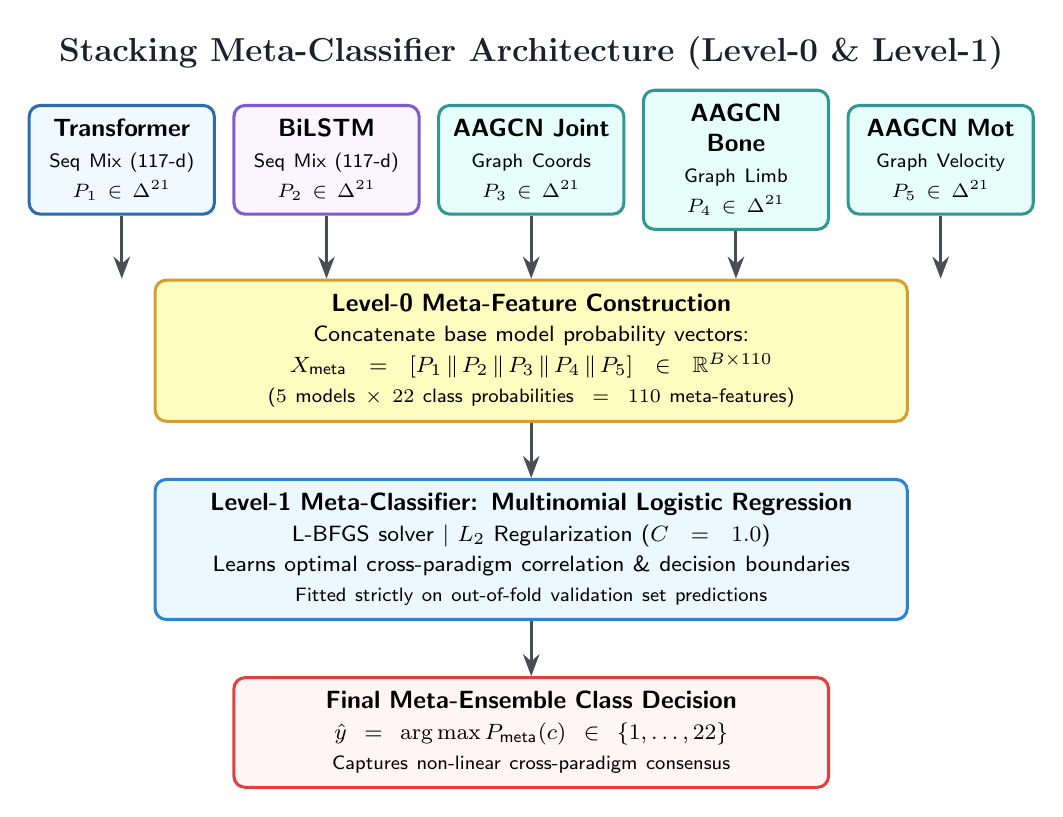
\begin{tikzpicture}[
    font=\sffamily\small,
    >=Stealth,
    node distance=0.65cm,
    block/.style={
        draw=#1,
        line width=1.1pt,
        rounded corners=4pt,
        align=center,
        inner sep=5pt
    },
    arrow/.style={->, line width=1.1pt, color=tDark!80}
]

\node[font=\bfseries\large, text=tDark] (title) at (6.0, 1.35) {Stacking Meta-Classifier Architecture (Level-0 \& Level-1)};

\node[block=bTrans, fill=cTrans, text width=2.0cm] (m1) at (0.8, 0) {
    \textbf{Transformer}\\
    {\scriptsize Seq Mix (117-d)}\\
    {\scriptsize $P_1 \in \Delta^{21}$}
};
\node[block=bRecurr, fill=cRecurr, text width=2.0cm] (m2) at (3.4, 0) {
    \textbf{BiLSTM}\\
    {\scriptsize Seq Mix (117-d)}\\
    {\scriptsize $P_2 \in \Delta^{21}$}
};
\node[block=bGCN, fill=cGCN, text width=2.0cm] (m3) at (6.0, 0) {
    \textbf{AAGCN Joint}\\
    {\scriptsize Graph Coords}\\
    {\scriptsize $P_3 \in \Delta^{21}$}
};
\node[block=bGCN, fill=cGCN, text width=2.0cm] (m4) at (8.6, 0) {
    \textbf{AAGCN Bone}\\
    {\scriptsize Graph Limb}\\
    {\scriptsize $P_4 \in \Delta^{21}$}
};
\node[block=bGCN, fill=cGCN, text width=2.0cm] (m5) at (11.2, 0) {
    \textbf{AAGCN Mot}\\
    {\scriptsize Graph Velocity}\\
    {\scriptsize $P_5 \in \Delta^{21}$}
};

% Meta-Features Formation
\node[block=bFusion, fill=cFusion, text width=9.2cm, below=0.8cm of m3] (meta) {
    \textbf{Level-0 Meta-Feature Construction}\\
    {\footnotesize Concatenate base model probability vectors:}\\
    {\footnotesize $X_{\text{meta}} = [P_1 \,\|\, P_2 \,\|\, P_3 \,\|\, P_4 \,\|\, P_5] \in \mathbb{R}^{B \times 110}$}\\
    {\scriptsize ($5 \text{ models} \times 22 \text{ class probabilities} = 110 \text{ meta-features}$)}
};

\draw[arrow] (m1.south) -- (meta.north -| m1.south);
\draw[arrow] (m2.south) -- (meta.north -| m2.south);
\draw[arrow] (m3) -- (meta);
\draw[arrow] (m4.south) -- (meta.north -| m4.south);
\draw[arrow] (m5.south) -- (meta.north -| m5.south);

% Level-1 Meta-Learner
\node[block=bInput, fill=cInput, text width=9.2cm, below=0.7cm of meta] (lr) {
    \textbf{Level-1 Meta-Classifier: Multinomial Logistic Regression}\\
    {\footnotesize L-BFGS solver \textbar{} $L_2$ Regularization ($C=1.0$)}\\
    {\footnotesize Learns optimal cross-paradigm correlation \& decision boundaries}\\
    {\scriptsize Fitted strictly on out-of-fold validation set predictions}
};

\draw[arrow] (meta) -- (lr);

% Final Output
\node[block=bHead, fill=cHead, text width=7.2cm, below=0.7cm of lr] (pred) {
    \textbf{Final Meta-Ensemble Class Decision}\\
    {\footnotesize $\hat{y} = \arg\max P_{\text{meta}}(c) \in \{1, \dots, 22\}$}\\
    {\scriptsize Captures non-linear cross-paradigm consensus}
};

\draw[arrow] (lr) -- (pred);

\end{tikzpicture}
\end{document}
